\def \Subject {گام سوم: کامل کردن تحقیقات راجع به موضوع}
\section{\Subject}
پس از انتخاب و تایید موضوع به تحقیقات بیشتر پرداختم.
اطلاعات جمع آوری شده خودم را کامل کردم و به جستجوی بیشتر پرداختم.
در ادامه خلاصه ای از اطلاعات جمع آوری شده را می‌توانید مشاهده کنید:

\begin{itemize}
\item 
{
Zigbee
چیست؟ 

ZigBee یک پروتکل ارتباطی بی‌سیم است که برای مصرف کم انرژی و نرخ داده پایین طراحی شده است. این پروتکل هزینه کمی دارد و قابل اعتماد است و به طور متداول در برنامه‌های اینترنت اشیاء (IoT) استفاده می‌شود. برد فیزیکی آن کوتاه است و بر اساس استاندارد 
802.15.4 IEEE 
استوار است. این پروتکل ارتباطی بی‌سیم ساده و قابل اعتمادی است که از سنسورها، سوئیچ‌ها و کنترل‌کننده‌ها و سایر دستگاه‌ها استفاده می‌کند. علاوه بر این، ZigBee به راحتی می‌تواند با سایر پروتکل‌های ارتباطی مانند Wi-Fi و بلوتوث یکپارچه شود. ZigBee در سال ۱۹۹۸ مطرح شد، در سال ۲۰۰۳ استانداردسازی شد و در سال ۲۰۰۶ بازبینی و به‌روزرسانی شد.
}

\item  
{
دلیل نامگذاری آن چیست؟

نام به رقص زنبور عسل پس از بازگشت به لانه اشاره دارد.
}

\item 
{
چرا ZigBee بوجود آمد؟

ZigBee برای پاسخ به نیاز به استاندارد ارتباطی بی‌سیمی ساخته شد که بتواند اتصال پایدار و کم‌مصرفی را برای دستگاه‌ها در مجموعه‌ای از برنامه‌ها فراهم کند. توسعه ZigBee تحت تأثیر خواسته برای ایجاد پروتکل بی‌سیمی بود که بتواند:
    \begin{itemize}
        \item {
            با مصرف کم انرژی عمل کند: ZigBee برای کار با مصرف بسیار پایین انرژی طراحی شده است و امکان اجرای دستگاه‌ها با باتری برای مدت زمان طولانی را فراهم می‌کند.
        }
        \item {
            تعداد زیادی دستگاه را پشتیبانی کند: ZigBee برای پشتیبانی از تعداد زیادی دستگاه طراحی شده است که بتوانند در شبکه مش به یکدیگر ارتباط برقرار کنند.
        }
        \item {
            نصب و نگهداری آسانی داشته باشد: ZigBee برای نصب و نگهداری آسان با پیکربندی و مدیریت ساده شبکه طراحی شده است.
        }
        \item {
            ارتباط قابل اعتماد را فراهم کند: ZigBee برای ارائه ارتباط قابل اعتماد، حتی در محیط‌هایی با سطوح بالای تداخل، طراحی شده است.
        }
        \item {
            انواع مختلفی از برنامه‌ها را پشتیبانی کند: ZigBee برای پشتیبانی از طیف وسیعی از برنامه‌ها، از جمله خانه‌های هوشمند، کنترل صنعتی و پایش سلامتی، طراحی شده است.
            به طور کلی، ZigBee برای برآورده کردن نیازهای خاص ارتباط بی‌سیمی کم‌مصرف و با نرخ داده کم برای دستگاه‌های IoT با تمرکز بر روی قابلیت اعتماد و اطمینان، قابلیت مقیاس‌پذیری و 
            سهولت استفاده توسعه یافته است.
        }

    \end{itemize}

}

\item {
    کاربرد های Zigbee چیست؟

    ZigBee یک فناوری ارتباط بی سیم محبوب است که کاربردهای گسترده ای در صنایع مختلف دارد. در اینجا برخی از کاربردهای رایج ZigBee آورده شده است:
    \begin{itemize}
        \item {
            اتوماسیون خانگی: ZigBee به طور گسترده در سیستم های اتوماسیون خانگی برای کنترل چراغ ها، سیستم های HVAC، قفل درها و سایر دستگاه ها استفاده می شود.
        }
        \item {
            اتوماسیون صنعتی: ZigBee در سیستم های اتوماسیون صنعتی برای نظارت و کنترل تجهیزات و ماشین آلات استفاده می شود.
        }
        \item {
            مراقبت های بهداشتی: ZigBee در برنامه های مراقبت های بهداشتی برای نظارت بر بیمار، ردیابی دارایی و تشخیص از راه دور استفاده می شود.
        }
        \item {
            شبکه هوشمند: ZigBee در سیستم های شبکه هوشمند برای کنترل و نظارت بر مصرف انرژی در خانه ها و ساختمان ها استفاده می شود.
        }
        \item {
            اتوماسیون ساختمان: ZigBee در سیستم های اتوماسیون ساختمان برای کنترل روشنایی، HVAC و سیستم های امنیتی استفاده می شود.
        }
        \item {
            پایش محیطی: ZigBee در سیستم های نظارت محیطی برای نظارت بر دما، رطوبت و کیفیت هوا استفاده می شود.
        }
        \item {
            کشاورزی: ZigBee در کاربردهای کشاورزی برای نظارت بر رطوبت خاک، دما و سایر پارامترها برای بهینه سازی عملکرد محصول استفاده می شود.
        }
        \item {
            حمل و نقل: ZigBee در برنامه های حمل و نقل برای ارتباط وسیله نقلیه به وسیله نقلیه و وسیله نقلیه به زیرساخت استفاده می شود.
        }

    \end{itemize}
}

\item {
    انواع دستگاه های Zigbee کدام اند؟

    \begin{itemize}
        \item {
            Coordinator ZigBee
            :
            Coordinator ZigBee
            دستگاه مرکزی در شبکه است که مسئول راه اندازی و مدیریت شبکه است. تنها یک Coordinator در شبکه وجود دارد و وظیفه تخصیص آدرس های شبکه به دستگاه های دیگر، تعریف پارامترهای شبکه و کنترل ترافیک شبکه را بر عهده دارد.
        }
        \item {
            Router
            ZigBee
            :
            روترهای ZigBee دستگاه های میانی هستند که داده ها را بین دستگاه های موجود در شبکه هدایت می کنند. آنها همچنین می توانند به عنوان نقاط پایانی عمل کنند که می توانند داده ها را دریافت یا انتقال دهند.
        }
        \item {
            Device End ZigBee  
            : 
            Devices 
            End 
            ZigBee 
            دستگاه هایی هستند که فقط از طریق روترها یا Coordinator می توانند با دستگاه های دیگر در شبکه ارتباط برقرار کنند. دستگاه‌های پایانی معمولاً قدرت پردازش و حافظه محدودی دارند و برای مصرف انرژی بسیار کم طراحی شده‌اند.
        }
    \end{itemize}

    \begin{figure}[H]
        \centering
        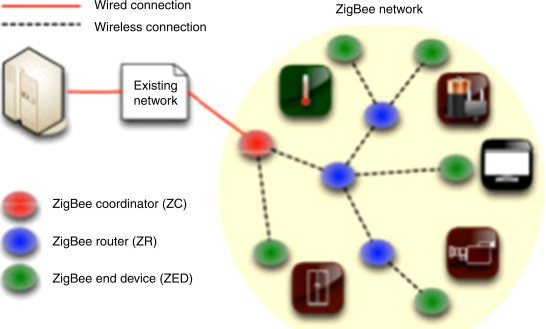
\includegraphics[width=0.65\linewidth]{images/device_types.jpg}
        \caption{ انواع دستگاه های Zigbee }
        \label{fig:h}
    \end{figure}

}

\item {
    معماری شبکه Zigbee چگونه است؟
    
    ZigBee از انواع مختلفی از توپولوژی های شبکه پشتیبانی می کند که امکان استقرار انعطاف پذیر دستگاه ها را در برنامه های مختلف فراهم می کند. توپولوژی های اصلی ZigBee عبارتند از:

    \begin{itemize}
        \item {
            Topology Star
            :
            در توپولوژی ستاره، همه دستگاه ها با یک گره مرکزی ارتباط برقرار می کنند که معمولاً هماهنگ کننده ZigBee است. این توپولوژی برای کاربردهایی که دستگاه ها در مجاورت هماهنگ کننده قرار دارند مناسب است.        }
        \item {
            Topology Mesh
            :
            در توپولوژی مش، دستگاه ها از طریق مسیرهای متعدد به هم متصل می شوند و داده ها را می توان از طریق هر مسیر موجود هدایت کرد. این توپولوژی قابلیت اطمینان شبکه بیشتری را فراهم می کند و برای برنامه هایی که دستگاه ها در یک منطقه بزرگتر پخش شده اند مناسب است.        }
        \item {
            Topology Tree  
            : 
            در توپولوژی درختی، دستگاه ها در یک ساختار سلسله مراتبی با هماهنگ کننده ZigBee در ریشه و سایر دستگاه ها از آن منشعب می شوند، سازماندهی می شوند. این توپولوژی برای کاربردهایی که دستگاه ها در فواصل مختلف از هماهنگ کننده قرار دارند مناسب است.    
            }
    \end{itemize}

    \begin{figure}[H]
        \centering
        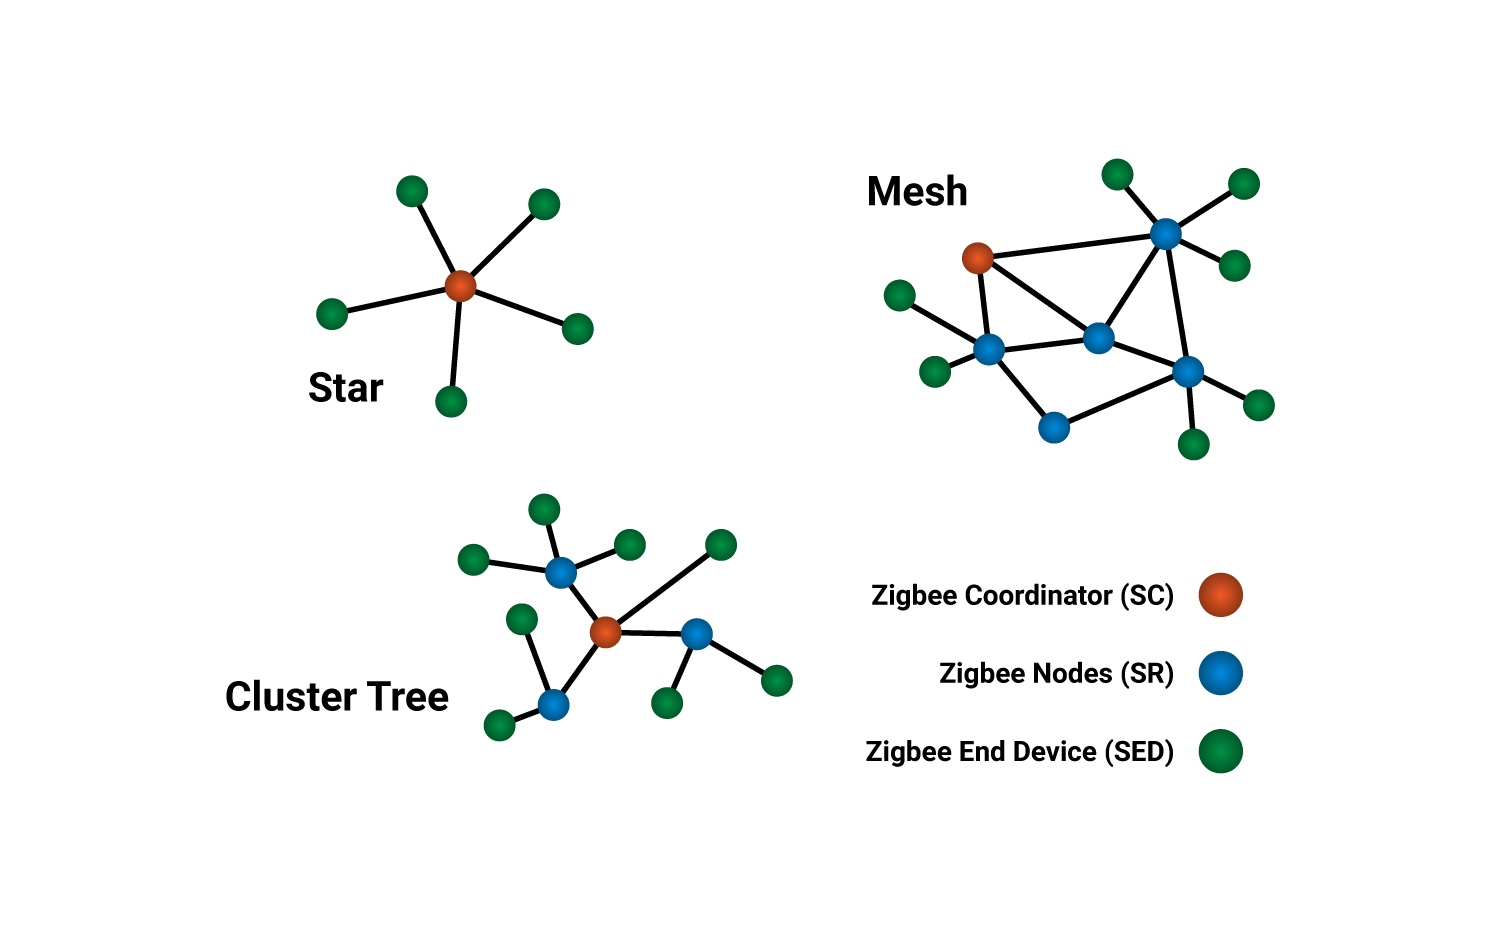
\includegraphics[width=1\linewidth]{images/topologies.jpg}
        \caption{ انواع توپولوژی های شبکه Zigbee }
        \label{fig:h}
    \end{figure}
}

\item {
    لایه های شبکه Zigbee چگونه است؟

    پروتکل ZigBee در لایه هایی سازماندهی شده است که عملکردها و خدمات مختلفی را ارائه می دهد. در اینجا لایه های پروتکل ZigBee آمده است:

    \begin{itemize}
        \item {
            layer Application 
            :
            این لایه عملکرد و خدمات در سطح برنامه مانند کشف دستگاه، جفت شدن دستگاه و انتقال داده را تعریف می کند. این یک رابط بین شبکه ZigBee و برنامه در حال اجرا در بالای آن فراهم می کند.
        }
        \item {
            layer Network 
            :
            این لایه عملکرد مدیریت شبکه مانند مسیریابی و آدرس دهی را فراهم می کند. وظیفه کشف مسیر بهینه برای انتقال داده و حفظ توپولوژی شبکه را بر عهده دارد.
        }
        \item {
            layer MAC   
            : 
            این لایه رابط بین لایه فیزیکی و لایه شبکه را فراهم می کند. مسئول مدیریت ارتباط بین گره ها از جمله دسترسی به کانال، قاب بندی داده ها و تشخیص خطا است.
            }
        \item {
            layer PHY  
            : 
            این لایه رابط فیزیکی بین دستگاه ZigBee و فرستنده فرکانس رادیویی (RF) را فراهم می کند. وظیفه انتقال و دریافت اطلاعات از طریق هوا را بر عهده دارد.
            هر لایه در پروتکل ZigBee مجموعه ای از توابع و خدمات خاص خود را دارد که با هم کار می کنند تا ارتباطات بی سیم قابل اعتماد و کم مصرف را برای برنامه های مختلف ارائه دهند.
            
            }
    \end{itemize}

    \begin{figure}[H]
        \centering
        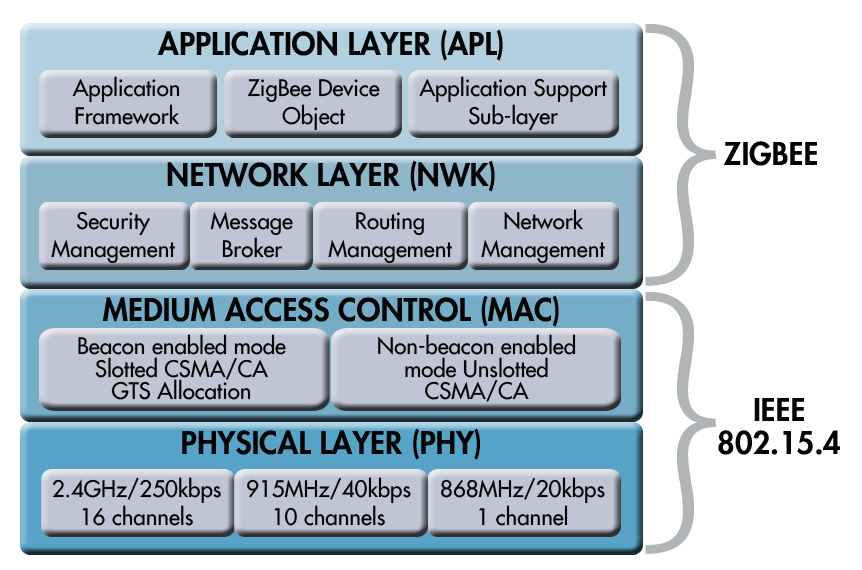
\includegraphics[width=1\linewidth]{images/layers.jpg}
        \caption{ لایه های شبکه Zigbee }
        \label{fig:h}
    \end{figure}
}

\item {
    ویژگی های امنیتی Zigbee چگونه است؟

    شبکه ZigBee از چندین ویژگی امنیتی از جمله رمزگذاری، احراز هویت و کنترل دسترسی پشتیبانی می کند تا از محرمانه بودن و یکپارچگی داده های منتقل شده از طریق شبکه اطمینان حاصل کند. اتحاد ZigBee که مسئولیت توسعه استاندارد ZigBee را بر عهده دارد، دستورالعمل ها و مشخصاتی را برای پیاده سازی امنیت در شبکه های ZigBee ارائه می دهد.

    همچنین Zigbee از 
    مکانیزم رمزگذاری AES-128 برای ایمن سازی ارتباط بین گره ها
    استفاده میکند.

}


\end{itemize}








